\begin{frame}{Dynamic Filter}
\begin{center}
	\scalebox{0.5}{
	  \Large
	  \tikzstyle{block} = [draw, left color=gray, right color= white, draw=gray!50!white]
	  \begin{tikzpicture}
	    \node [block] at (0,0) (lipm) {
        LIPM
      };
      	\node [block] at ([yshift=-2cm]lipm) (ik) {
        Analytical Inverse Kinematics
      };
      \draw [->] (lipm) -- node[right] {CoM$_{\text{LIPM}}$, Feet} (ik) ;
      	\node [block] at ([yshift=-2cm]ik) (id) {
        RNEA Inverse Dynamics
      };
      \draw [->] (ik) -- node[right] {$\mq$, $\mqdot$, $\mqddot$} (id) ;
      \node [block] at ([yshift=-2cm]id) (sub) {
        CoP$_{\text{LIPM}}$ - CoP$_{\text{MB}}$
      };
      \draw [->] (id) -- node[right] {CoP$_{\text{MB}}$} (sub) ;
      \draw [- ] (lipm.east) -| node[xshift=1cm,yshift=-3cm]{CoP$_{\text{LIPM}}$} ([xshift=3cm]sub.east) ;
      \draw [->] ([xshift=3cm]sub.east) -- (sub.east) ;
      \node [block] at ([yshift=-2cm]sub) (oc) {
        Approximation of : $CoM = F(CoP)$
      };
      \draw [->] (sub) -- node[right] {$\Delta$CoP} (oc) ;
      \node [block] at ([yshift=-2cm]oc) (add) {
        CoM$_{\text{MB}}$ = CoM$_{\text{LIPM}}$ + $\Delta$CoM
      };
      \draw [->] (oc) -- node[right] {$\Delta$CoM} (add) ;
      \draw [->] (add) -- node[right] {CoM$_{\text{MB}}$, Feet, CoP$_{\text{LIPM}}$} ([yshift=-2cm]add.south) ;
      
      \draw [- ] (lipm.west) -| node[xshift=-1cm,yshift=-5cm]{CoM$_{\text{LIPM}}$} ([xshift=-2cm]add.west) ;
      \draw [->] ([xshift=-2cm]add.west) -- (add.west) ;
      
		\end{tikzpicture}
  }
\end{center}
\end{frame}

%%%%%%%%%%%%%%%%%%%%%%%%%%%%%%%%%%%%%%%%%%%%%%%%%%%%%%%%%%%%%%%%%%%%%%%%%%%%%%%%%%%%%%%%%
\begin{frame}{Dynamic Filter}
\vspace*{-1cm}
  \begin{center}
    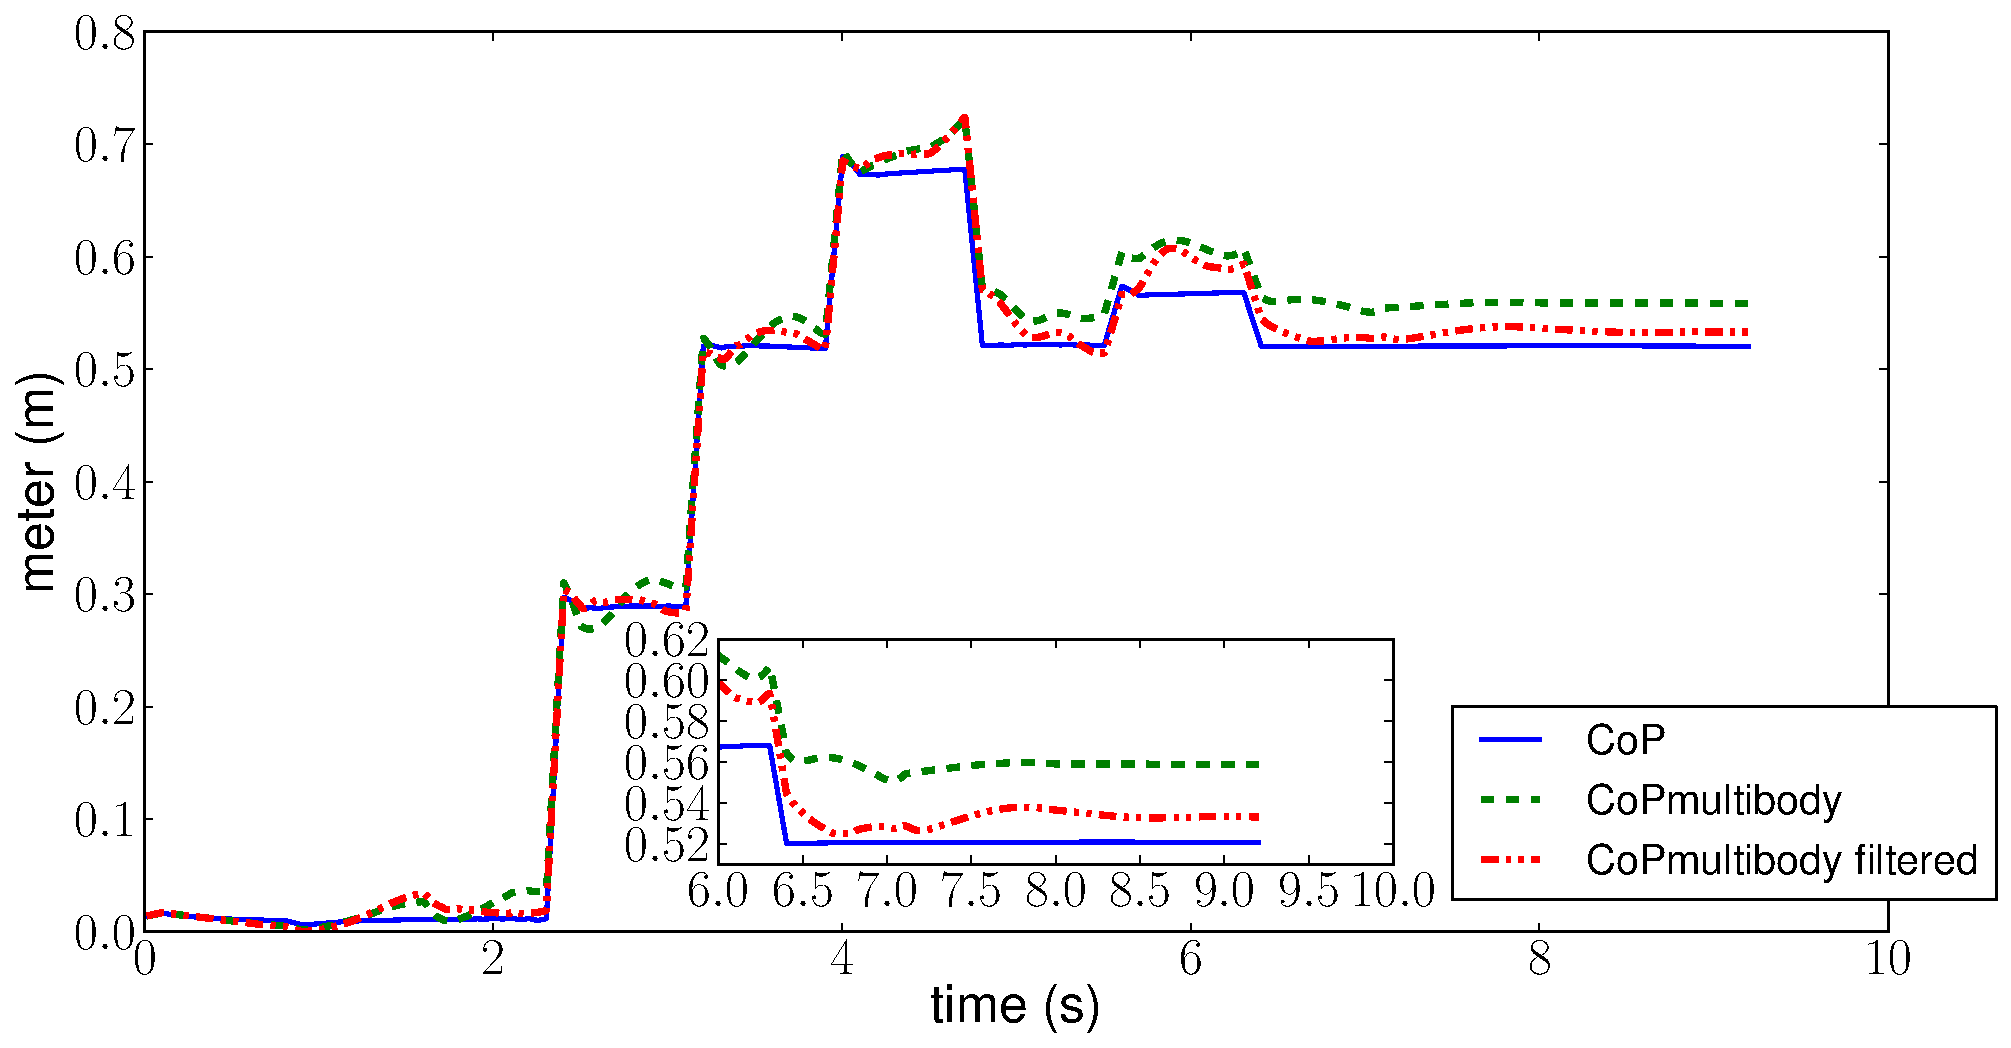
\includegraphics[height=0.7\textheight, keepaspectratio]
      {./figures/nmpc_walkgen/copmbpres.pdf}    
  \end{center}
\end{frame}

%%%%%%%%%%%%%%%%%%%%%%%%%%%%%%%%%%%%%%%%%%%%%%%%%%%%%%%%%%%%%%%%%%%%%%%%%%%%%%%

\begin{frame}{Experiment on HRP2}
  \begin{center}
    \movie[autostart,loop]{
    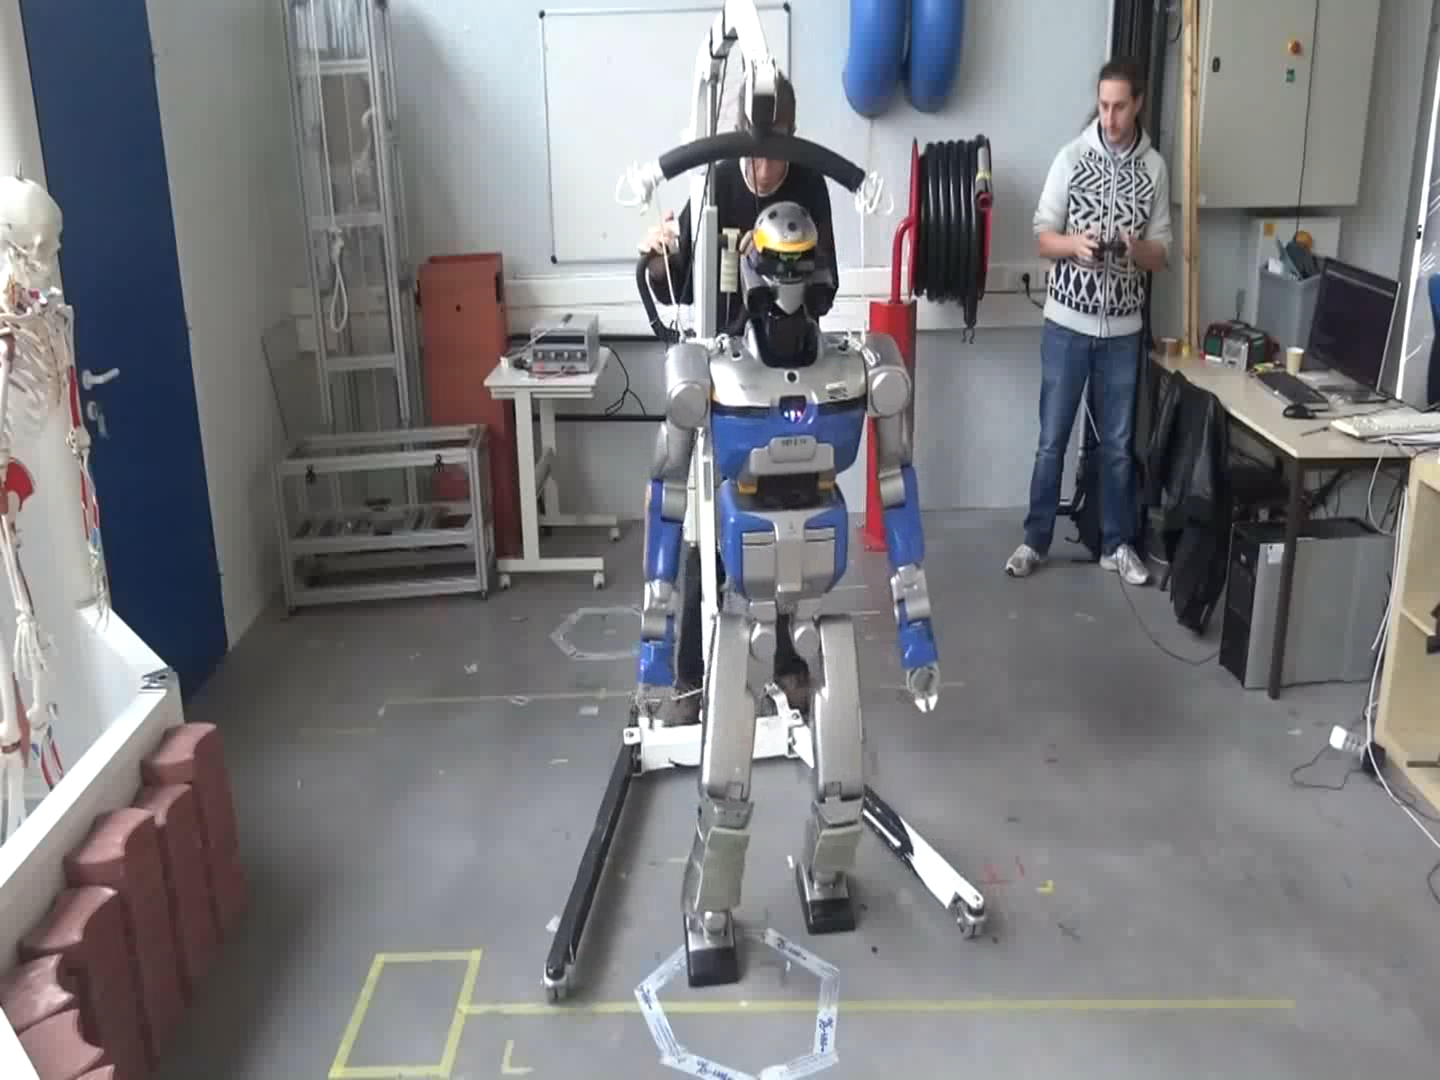
\includegraphics[height=0.7\textheight, aspectratio=43]
      {dynfilt.png}    
    }  
    {videos/dynfilt.mp4}
  \end{center}
  \vspace*{-0.5cm}
\blfootnote{\textbf{Naveau}, Stasse et al., Humanoids 2014}
\end{frame}

%%%%%%%%%%%%%%%%%%%%%%%%%%%%%%%%%%%%%%%%%%%%%%%%%%%%%%%%%%%%%%%%%%%%%%%%%%%%%%%
